\section{Resultados Experimentales y Análisis Estadístico}\label{sec:results}

\subsection{Métricas de clasificación sobre el conjunto de prueba}
El modelo campeón se evaluó sobre el conjunto de prueba
($N_{test}=334\,566$), que permaneció aislado durante todo el proceso de
optimización. La Tabla~\ref{tab:classreport} presenta el reporte de clasificación
completo, generado con cuatro decimales de precisión.

\begin{table}[H]
\centering
\caption{Reporte de clasificación sobre el conjunto de prueba}
\label{tab:classreport}
\footnotesize
\begin{tabular}{lcccc}
\toprule
\textbf{Clase} & \textbf{Precision} & \textbf{Recall} & \textbf{F1-Score} & \textbf{Soporte} \\
\midrule
0 (Normal) & 0.9835 & 0.8859 & 0.9322 & 280\,224 \\
1 (Helada) & 0.6109 & 0.9234 & 0.7353 & 54\,342 \\
\midrule
\textit{Accuracy} & \multicolumn{3}{c}{0.8920} & 334\,566 \\
\textit{Macro avg} & 0.7972 & 0.9047 & 0.8338 & 334\,566 \\
\textit{Weighted avg} & 0.9230 & 0.8920 & 0.9002 & 334\,566 \\
\bottomrule
\end{tabular}
\end{table}

El modelo alcanzó un \emph{Recall} de $92.34\%$ para la clase minoritaria
(helada), a costa de una \emph{Precision} de $61.09\%$ en dicha clase. Este
compromiso es deliberado y coherente con el objetivo operativo de minimizar los
falsos negativos en un contexto de prevención de desastres agrometeorológicos:
en un sistema de alerta temprana, omitir una helada real (falso negativo) tiene un
costo agrícola muy superior al de emitir una alerta que no se materializa (falso
positivo).

\subsection{Métricas globales robustas al desbalance}
Dado el desbalance de clases documentado en la Sección~\ref{sec:dataset}, se
reportan métricas específicamente robustas frente a distribuciones asimétricas.
La Tabla~\ref{tab:globalmetrics} consolida las métricas globales del modelo.

\begin{table}[H]
\centering
\caption{Métricas globales del modelo campeón}
\label{tab:globalmetrics}
\footnotesize
\renewcommand{\arraystretch}{1.2}
\begin{tabular}{lc}
\toprule
\textbf{Métrica} & \textbf{Valor} \\
\midrule
Exactitud (\emph{Accuracy}) & 0.8920 \\
F1-Score Macro (validación interna, 3-fold) & 0.8330 \\
F1-Score Macro (conjunto de prueba) & 0.8338 \\
Índice Kappa de Cohen ($\kappa$) & 0.6710 \\
Área bajo la curva ROC (ROC-AUC) & 0.9690 \\
\bottomrule
\end{tabular}
\end{table}

El índice Kappa de Cohen de $\kappa=0.6710$ indica una concordancia
\emph{sustancial} entre las predicciones y las etiquetas reales, según la escala
de interpretación convencional, descontando los aciertos atribuibles al azar. El
área bajo la curva ROC de $0.9690$ evidencia una elevada capacidad discriminante
global del clasificador. La estrecha correspondencia entre el F1-Score Macro de
validación interna ($0.8330$) y el de prueba ($0.8338$) sugiere ausencia de
sobreajuste significativo y buena capacidad de generalización.

\subsection{Matriz de confusión y curvas de desempeño}
La Fig.~\ref{fig:eval} presenta, de izquierda a derecha, la matriz de confusión,
la curva ROC y la curva Precision-Recall obtenidas sobre el conjunto de prueba.
La curva Precision-Recall es particularmente informativa en escenarios
desbalanceados, ya que evalúa directamente la capacidad de aislar la clase
minoritaria sin verse favorecida por el gran volumen de verdaderos negativos.

\begin{figure*}[t]
\centering
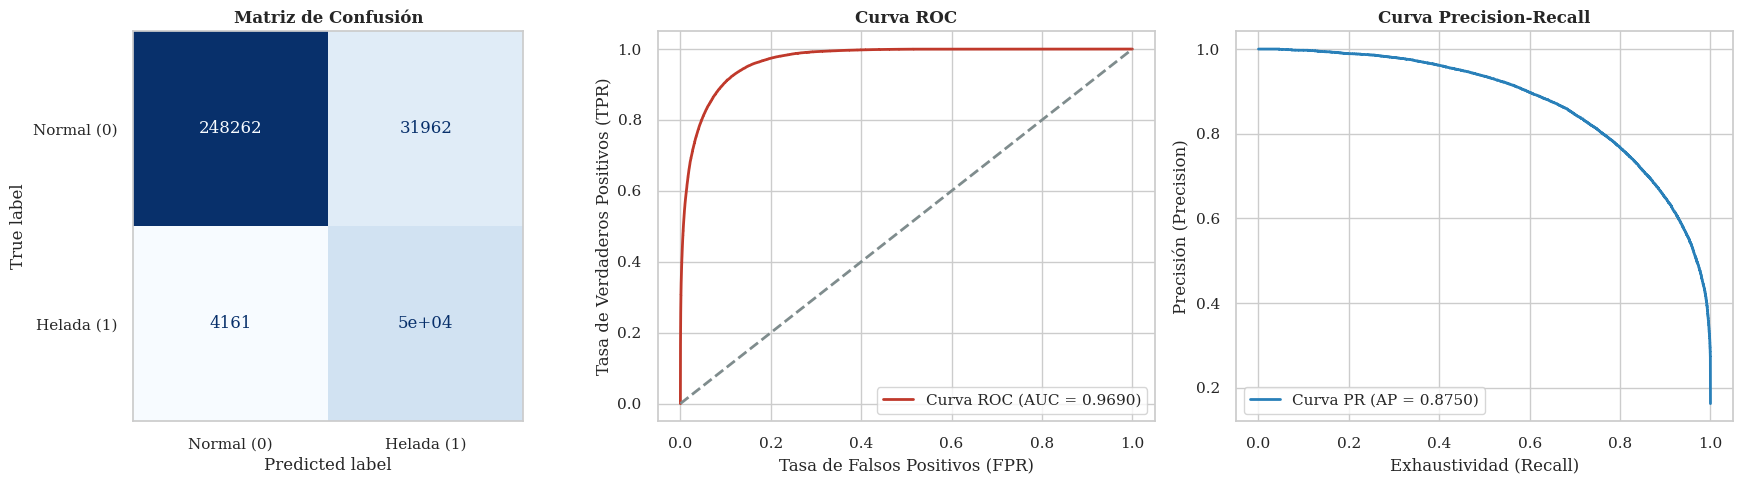
\includegraphics[width=0.95\textwidth]{img/cell19_out1.png}
\caption{Evaluación integral del modelo campeón sobre el conjunto de prueba:
matriz de confusión (izquierda), curva ROC con AUC$=0.9690$ (centro) y curva
Precision-Recall (derecha).}
\label{fig:eval}
\end{figure*}

\subsection{Importancia de los componentes principales}
La Fig.~\ref{fig:importance} presenta la reducción media de impureza de Gini
atribuida a cada componente principal por el ensamble. El hallazgo más relevante
es que la capacidad discriminante del modelo no reside en la dirección de mayor
varianza global (PC1), sino en componentes latentes ortogonales específicos,
identificados como PC3 y PC2. Esto revela que la señal predictiva de la helada
habita en direcciones de varianza intermedia y no en la dominante, un resultado
no trivial desde la perspectiva del análisis espectral.

\begin{figure}[H]
\centering
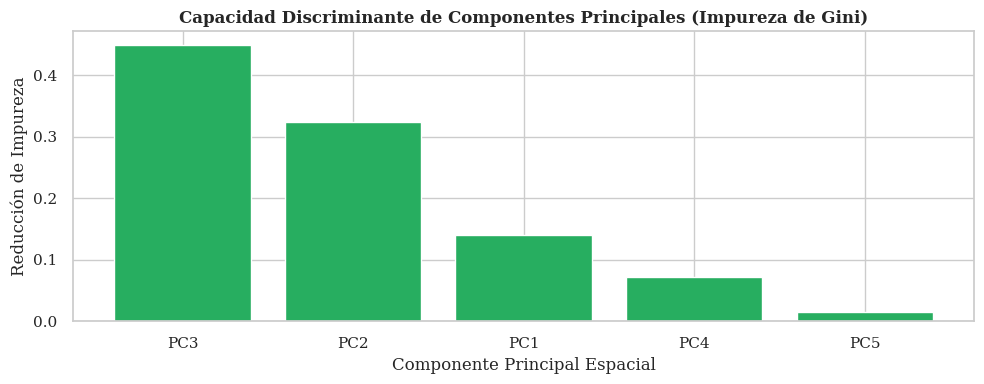
\includegraphics[width=0.90\textwidth]{img/cell19_out2.png}
\caption{Capacidad discriminante (impureza de Gini) de los componentes
principales empleados por el modelo campeón.}
\label{fig:importance}
\end{figure}

\subsection{Análisis estadístico de significancia}
El diseño experimental documentado no permite realizar un análisis estadístico
inferencial de significancia. La aplicación de pruebas como la de Wilcoxon
(comparación pareada de dos modelos), ANOVA (comparación de tres o más modelos) o
el procedimiento post-hoc de Tukey requiere dos condiciones que el pipeline actual
no satisface: (i) la existencia de \emph{múltiples modelos de línea base}
entrenados bajo protocolo idéntico para su contraste, y (ii) la disponibilidad de
\emph{múltiples ejecuciones independientes} por modelo (p.\,ej. mediante semillas
distintas o validación cruzada repetida) que provean las distribuciones de
métricas sobre las cuales aplicar dichas pruebas.

En su estado actual, el experimento entrena un único modelo (Random Forest
optimizado) con una semilla fija ($\text{SEED}=42$) y lo evalúa una sola vez sobre
un único conjunto de prueba. En consecuencia:

\begin{quote}
\emph{El análisis estadístico inferencial no pudo realizarse debido a que el
notebook no conserva múltiples ejecuciones independientes necesarias para aplicar
pruebas de significancia.}
\end{quote}

Para habilitar este análisis en trabajos futuros, se propone el siguiente
protocolo experimental: (1) entrenar un conjunto de modelos de línea base
(p.\,ej. Regresión Logística, SVM, XGBoost) bajo el mismo pipeline de
preprocesamiento; (2) ejecutar validación cruzada estratificada de $k$ particiones
repetida $r$ veces con semillas distintas, registrando el F1-Score Macro de cada
repetición; (3) aplicar la prueba de Friedman para detectar diferencias globales
entre modelos y, de resultar significativa, el post-hoc de Nemenyi (o Wilcoxon con
corrección de Bonferroni para comparaciones pareadas contra el modelo propuesto).
Este diseño proporcionaría la evidencia estadística necesaria para afirmar que las
diferencias de rendimiento no son producto del azar experimental.